\subsubsection{ボリューム}\label{volume}
\begin{table}[H]
  \begin{widerrows}
    \begin{tabular}{|p{\colF}|p{\colG}|}	\hline
    名称 & ボリューム(ぼりゅーむ)\\ \hline
    接続箇所 & アナログコネクタ (3pin)\\ \hline
    機能概要 & つまみの回転量を出力\\ \hline
    \end{tabular}
  \end{widerrows} 
\end{table}

\begin{table}[H]
  \begin{widerrows}
    \begin{tabular}{|p{\colF}|p{\colG}|}	\hline
    サンプルコードの場所 & 05/anain.hsp\\ \hline
    raspiへの入力 & つまみの回転量 0から1023の値\\ \hline
    raspiへの入力方法 & 力を入れすぎて壊れないよう注意\\ \hline
    raspiからの出力 & なし\\ \hline
    raspiからの出力方法 & なし\\ \hline
    \end{tabular}
  \end{widerrows} 
\end{table}

\begin{figure}[H]
  \begin{widerrows}
    \begin{tabular}{|p{\colF}|p{\colG}|} \hline
    使い道 & 音量調整, LEDの明るさ調整, ゲームのコントローラとして\\ \hline
    注意事項 & 強く押して壊さないように注意\\ \hline
    補足 & 先端のつまみをつまんで回転させると\ruby{抵抗値}{てい|こう|ち}が変化しraspberry piに入力される電圧が変化します。今回使うボリュームは左に回しきったときは変化が小さく、右に回すほど変化が大きくなります(指数関数的)。この設定をAカーブと呼びます (図\ref{ボリュームの特性})。これはボリュームがしばしば音量調節に利用され、人間の耳の感度は対数関数的(小さい音ほど\ruby{敏感}{びん|かん}で大きい音に関しては\ruby{鈍感}{どん|かん})であることからこのように設定されています。もちろん、ボリュームは音量調節以外にも使用されるため、\ruby{用途}{よう|と}に応じて特性が線形(傾きが一定)なBカーブや対数関数的(\ruby{傾}{かたむ}きが小さくなっていく)なCカーブなどが\ruby{存在}{そん|ざい}します。\par
  ボリュームには端子が3つ付いており、図\ref{ボリュームの仕組み}のように1つに+\ruby{電源}{でん|げん}を、1つに-電源をつなげ、もう1つを出力として使用します。+電源から-電源までに\ruby{帯状}{おび|じょう}の抵抗器が接続されており、その間に出力の端子が接続されています。シャフトを回すことで、出力端子の位置が変化し、結果プラス電源端子-出力端子間と出力端子-マイナス電源端子間の抵抗値が変化することになります。
    \begin{minipage}[t]{0.45\linewidth}
      \smallskip
        \centering
        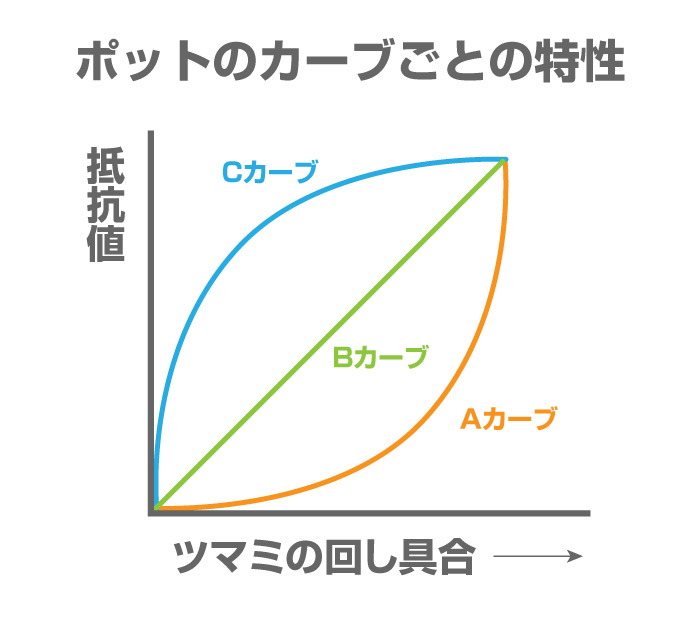
\includegraphics[width=\linewidth]{images/chap05/text05-img050.jpg}
        \caption{ボリュームの特性}
        \label{ボリュームの特性}
        \smallskip
      \end{minipage}
      \begin{minipage}[t]{0.45\linewidth}
      \smallskip
        \centering
        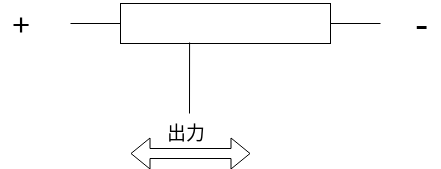
\includegraphics[width=\linewidth]{images/chap05/text05-img051.png}
        \caption{ボリュームの仕組み}
        \label{ボリュームの仕組み}
        \smallskip
      \end{minipage}\\ \hline
    \end{tabular}
  \end{widerrows} 
\end{figure}

\begin{figure}[H]
  \begin{widerrows}
    \begin{tabular}{|p{\colH}|p{\colI}|p{\colH}|p{\colI}|} \hline
    外観 & 
    \begin{minipage}[t]{\linewidth}
      \smallskip
        \centering
        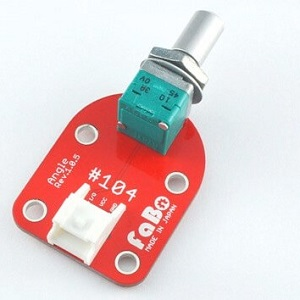
\includegraphics[width=0.5\linewidth]{images/chap05/text05-img022.jpg}
        \caption{ボリューム}
        \smallskip
      \end{minipage} &
      回路記号 & 
      \begin{minipage}[t]{\linewidth}
      \smallskip
        \centering
        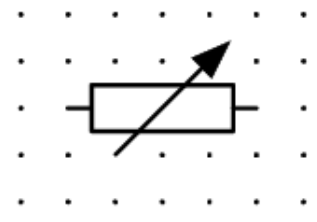
\includegraphics[width=0.5\linewidth]{images/chap05/text05-img052.png}
        \caption{ボリュームの回路図}
        \smallskip
      \end{minipage}\\ \hline
    \end{tabular}
  \end{widerrows} 
\end{figure}